% Options for packages loaded elsewhere
\PassOptionsToPackage{unicode}{hyperref}
\PassOptionsToPackage{hyphens}{url}
%
\documentclass[
]{book}
\usepackage{amsmath,amssymb}
\usepackage{iftex}
\ifPDFTeX
  \usepackage[T1]{fontenc}
  \usepackage[utf8]{inputenc}
  \usepackage{textcomp} % provide euro and other symbols
\else % if luatex or xetex
  \usepackage{unicode-math} % this also loads fontspec
  \defaultfontfeatures{Scale=MatchLowercase}
  \defaultfontfeatures[\rmfamily]{Ligatures=TeX,Scale=1}
\fi
\usepackage{lmodern}
\ifPDFTeX\else
  % xetex/luatex font selection
\fi
% Use upquote if available, for straight quotes in verbatim environments
\IfFileExists{upquote.sty}{\usepackage{upquote}}{}
\IfFileExists{microtype.sty}{% use microtype if available
  \usepackage[]{microtype}
  \UseMicrotypeSet[protrusion]{basicmath} % disable protrusion for tt fonts
}{}
\makeatletter
\@ifundefined{KOMAClassName}{% if non-KOMA class
  \IfFileExists{parskip.sty}{%
    \usepackage{parskip}
  }{% else
    \setlength{\parindent}{0pt}
    \setlength{\parskip}{6pt plus 2pt minus 1pt}}
}{% if KOMA class
  \KOMAoptions{parskip=half}}
\makeatother
\usepackage{xcolor}
\usepackage{longtable,booktabs,array}
\usepackage{calc} % for calculating minipage widths
% Correct order of tables after \paragraph or \subparagraph
\usepackage{etoolbox}
\makeatletter
\patchcmd\longtable{\par}{\if@noskipsec\mbox{}\fi\par}{}{}
\makeatother
% Allow footnotes in longtable head/foot
\IfFileExists{footnotehyper.sty}{\usepackage{footnotehyper}}{\usepackage{footnote}}
\makesavenoteenv{longtable}
\usepackage{graphicx}
\makeatletter
\def\maxwidth{\ifdim\Gin@nat@width>\linewidth\linewidth\else\Gin@nat@width\fi}
\def\maxheight{\ifdim\Gin@nat@height>\textheight\textheight\else\Gin@nat@height\fi}
\makeatother
% Scale images if necessary, so that they will not overflow the page
% margins by default, and it is still possible to overwrite the defaults
% using explicit options in \includegraphics[width, height, ...]{}
\setkeys{Gin}{width=\maxwidth,height=\maxheight,keepaspectratio}
% Set default figure placement to htbp
\makeatletter
\def\fps@figure{htbp}
\makeatother
\setlength{\emergencystretch}{3em} % prevent overfull lines
\providecommand{\tightlist}{%
  \setlength{\itemsep}{0pt}\setlength{\parskip}{0pt}}
\setcounter{secnumdepth}{5}
\usepackage{booktabs}
\ifLuaTeX
  \usepackage{selnolig}  % disable illegal ligatures
\fi
\usepackage[]{natbib}
\bibliographystyle{plainnat}
\IfFileExists{bookmark.sty}{\usepackage{bookmark}}{\usepackage{hyperref}}
\IfFileExists{xurl.sty}{\usepackage{xurl}}{} % add URL line breaks if available
\urlstyle{same}
\hypersetup{
  pdftitle={Bias within the AI Environment},
  pdfauthor={Drew, Grace, Vivi, Xinyan, Yibo},
  hidelinks,
  pdfcreator={LaTeX via pandoc}}

\title{Bias within the AI Environment}
\author{Drew, Grace, Vivi, Xinyan, Yibo}
\date{2023-08-15}

\begin{document}
\maketitle

{
\setcounter{tocdepth}{1}
\tableofcontents
}
\hypertarget{introduction}{%
\chapter{Introduction}\label{introduction}}

AI has increasingly become a topic of conversation, as it is a new technology with infinite possibilities. Since AI takes information from all over the internet, it is important to think about the biases that can be found within the system. For this project, we start by differentiating the difference between inaccuracy and biases. Specifically, we discuss AI/ML bias through the lens of machine model training biases - both unintentional and unintentional biases - also called inherent biases, as well as data collection biases, and the impact of these biases in the real world.

Through research, we hope to create a comprehensive understanding of bias within the AI space and how best to mitigate it as a user.

The project intends to create awareness about AI bias and help our Ross peers navigate the complex but crucial ethical aspect of AI. At the same time, a significant portion of the guide is dedicated to `responsible prompting', a practical guideline on crafting prompts mindfully and vigilantly spotting bias in AI responses. The goal of our project is to make AI interactions more fair, ethical, and responsible by empowering users to recognize and navigate AI biases.

In addition, the development of AI is also inseparable from Agile thinking. For example, we need to use Agile to continuously judge customer needs, just like the training mechanism of AI timely feedback. Agile methods emphasize rapid iteration during product development and gathering user feedback early on. This rapid iteration can make the team more acutely aware of potential ethical issues and make adjustments at an early stage. In the development and application of AI, especially in areas involving sensitive data or potential moral hazards, rapid iteration helps to detect and resolve possible ethical issues as early as possible. In a sense, AI and agility help each other. But the agile method itself does not ensure the ethics of AI, it is only a management and development method.

\hypertarget{about-us}{%
\chapter{About Us}\label{about-us}}

Introducing our exceptional team, a diverse and talented group of individuals, each with their own unique strengths and passions:

\hypertarget{grace}{%
\section*{Grace}\label{grace}}
\addcontentsline{toc}{section}{Grace}

I am a Master of Business Analytics Student at the Ross School of Business. I did my undergraduate degree at the University of Michigan School of Information, focusing on Information Analysis. I started a mental health club at the university called IfYou'reReadingThis. My interests include sports, fashion, and needlepoint.

\hypertarget{vivi}{%
\section*{Vivi}\label{vivi}}
\addcontentsline{toc}{section}{Vivi}

Experienced in crisis intervention and corporate cannabis. Combines passion for data analytics with industry insights as an MBAn student at UM Ross. Enjoys cooking and knitting for their 4 pets -- two dogs and two cats.

\hypertarget{yibo}{%
\section*{Yibo}\label{yibo}}
\addcontentsline{toc}{section}{Yibo}

Hi, I am Yibo
I am an accomplished international student from China who graduated in 2020 from the University of Connecticut, holding a dual major in Digital Marketing and Economics. Currently, I am pursuing my graduate studies in the Business Analysis Program at Umich Ross Business School.

\hypertarget{xinyan}{%
\section*{Xinyan}\label{xinyan}}
\addcontentsline{toc}{section}{Xinyan}

I arrived in the United States almost two months ago. Before this, I had been living in the beautiful southern city of Hangzhou, China, for 23 years. I have a Samoyed dog and a long-legged Napoleon cat. My hobbies involve photography and traveling, and I love exploring new things.

\hypertarget{drew}{%
\section*{Drew}\label{drew}}
\addcontentsline{toc}{section}{Drew}

Hello! I am currently a Master of Business Analytics Student at the Ross School of Business. I did my undergraduate degree at University of Michigan with majors in Mathematics and English and a minor in Physics. I was a writer and editor at the student publication The Michigan Daily. I love music, film, and running.

\hypertarget{as-a-team}{%
\section*{As a Team}\label{as-a-team}}
\addcontentsline{toc}{section}{As a Team}

Formed as a team for the class, MBAN 501: Software Teams and Project Management, we found ourselves sharing the same interest in the human processes that live behind the standard deliverables and tools used in business.

\hypertarget{overview-of-ai-biases}{%
\chapter{Overview of AI Biases}\label{overview-of-ai-biases}}

Insert intro here

\hypertarget{types-of-biases}{%
\section{Types of Biases}\label{types-of-biases}}

Insert types

\hypertarget{source-of-biases}{%
\section{Source of Biases}\label{source-of-biases}}

Insert sources

\hypertarget{examples}{%
\section{Examples}\label{examples}}

Insert examples

\hypertarget{overview-of-ai-and-llm}{%
\chapter{Overview of AI and LLM}\label{overview-of-ai-and-llm}}

\hypertarget{artificial-intelligence}{%
\section{Artificial Intelligence}\label{artificial-intelligence}}

Artificial Intelligence (AI) is a captivating field in computer science that aims to create systems capable of mimicking human intelligent behaviors. The history of this concept dates back to the mid-20th century when computer scientist Alan Turing introduced the famous Turing Test, defining AI as systems that exhibit actions ``like those of a human being.'' Despite controversies surrounding the Turing Test at the time, it laid the foundation for later AI research, defining AI as systems that can demonstrate human-like intelligence.

Stuart Russell and Peter Norvig, authors of ``Artificial Intelligence: A Modern Approach,'' identified four potential goals of AI, which influence its development direction. These goals differentiate AI systems based on their rationality and thinking versus acting:

\begin{enumerate}
\def\labelenumi{\arabic{enumi}.}
\tightlist
\item
  Systems that think like humans.
\item
  Systems that act like humans.
\item
  Systems that think rationally.
\item
  Systems that act rationally.
\end{enumerate}

These goals emphasize the positive impact of AI on human society and values, not just technological advancement.

At its simplest level, AI combines computer science with powerful data processing capabilities to address various problems. This field encompasses subfields like machine learning and deep learning, closely related to AI. Machine learning and deep learning involve training algorithms to recognize patterns and extract information from data. These methods have made significant progress in fields like image recognition, natural language processing, and recommendation systems. These algorithms build expert systems that predict, classify, and make decisions based on input data.

\hypertarget{narrow-ai}{%
\subsection{Narrow AI}\label{narrow-ai}}

Narrow AI, also known as Weak AI or Applied AI, refers to AI systems that focus on and can only solve specific domain problems. Most AI algorithms and applications we see today fall under the category of Narrow AI. Narrow AI excels in performing individual tasks. While these machines may appear intelligent, their capabilities are limited compared to even the most basic human intelligence.

In the realm of Narrow AI technology, research experience accumulated by humans and practices in engineering management and safety regulations often apply. Whether it's a self-driving car or a crane operator system, both require rigorous quality control processes and safety oversight strategies. Errors in autonomous driving programs could lead to accidents, just as mistakes in crane design could cause the crane to tip over, resulting in casualties. In essence, Narrow AI is merely a technological tool, and if it poses risks, they aren't fundamentally different from risks associated with widely-used technologies.

Examples of Narrow AI include chatgpt, virtual assistants like Siri and Alexa, self-driving cars, search engines like Google, conversational robots, spam filters, and Netflix recommendations.

\hypertarget{general-ai}{%
\subsection{General AI}\label{general-ai}}

General AI, also known as strong AI or Artificial General Intelligence (AGI), is a theoretical form of AI in which machines possess intelligence comparable to human beings. AGI is a concept wherein machines could have intelligence equivalent to human beings, encompassing self-awareness, problem-solving, learning, and future planning abilities. General AI can perform a variety of tasks across different domains and learn to solve new problems autonomously.

While Narrow AI focuses on performing specific tasks, such as answering questions based on user input or playing chess, AGI can perform a variety of functions and eventually learn to solve new problems on its own. Narrow AI relies on human intervention to define the parameters of its learning algorithms and provide relevant training data to ensure accuracy. Although human input accelerates the growth of AGI, it's not necessary, and over time, it could develop consciousness similar to human beings.

Strong AI possesses the following capabilities: Reasoning, strategizing, problem-solving, and decision-making in the presence of uncertainty. Knowledge representation, including common-sense knowledge. Planning. Learning. Communication through natural language. Integration of the above abilities to achieve set goals.

If computer programs could evolve to be smarter than the smartest and most gifted humans in the world, the resulting AI system could be referred to as Artificial Superintelligence (ASI). ASI is a theoretical concept representing an AI system with capabilities and potential far beyond human intelligence. Unlike existing Narrow AI and General AI (AGI), ASI is an immensely powerful and advanced form of intelligence.

\hypertarget{how-it-works}{%
\subsection{How It Works}\label{how-it-works}}

AI programming focuses on cognitive skills including learning (acquiring data and converting it into actionable information, i.e., algorithms), reasoning, self-correction, and creativity. The workflow of AI involves:

\textbf{Input:} Engineers gather the data needed for AI to operate normally, such as text, images, and speech. Ensuring that algorithms can read this input data is crucial. Contextualizing the data and defining the desired outcomes are important.

\textbf{Processing:} AI interprets the pre-programmed data and uses the
behaviors it has learned to recognize the same or similar behavior
patterns in real-time data.

\textbf{Data Outcomes:} Determining whether the data and its given
predictions are failures or successes.

\textbf{Adjustment:} If the dataset fails, AI can learn from the mistakes and repeat the process in a different way. The rules of the algorithm may need adjustments or changes to suit the dataset. This stage may see changes in outcomes to reflect more ideal or suitable results.

\textbf{Assessment:} Once AI completes the assigned task, the final step is assessment. This stage allows the technology to analyze the data and make inferences and predictions. It also provides useful feedback before running the algorithm again.

AI systems work by ingesting large amounts of labeled training data and combining rapid iterative processing with intelligent algorithms. They analyze the data's correlations and patterns, allowing software to learn patterns or features from data automatically. This way, a chatbot fed with examples of text conversations can learn to engage in convincing conversations, or an image recognition tool can learn to identify and describe objects in images by observing millions of examples. Emerging generative AI technologies create realistic text, images, music, and other media.

The core principle of AI is leveraging data-driven methods, deep
learning, and machine learning to process information, extract relevant patterns, and generate responses or outputs that resemble human intelligence.

\hypertarget{large-language-models}{%
\section{Large Language Models}\label{large-language-models}}

\hypertarget{how-it-works-1}{%
\subsection{How It Works}\label{how-it-works-1}}

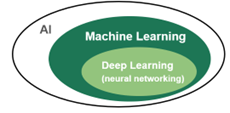
\includegraphics{lm.png}

Large Language Models (LLMs) utilize deep learning techniques, particularly neural networks, to comprehend and generate text similar to human natural language. These models are trained on extensive text data to capture language patterns, syntax, semantics, and context. The working mechanism of large language models involves but is not limited to the following steps:

\textbf{Tokenization:} Input text is divided into smaller units called
tokens, which can be words, subwords, or even characters, depending on the model's architecture and training data.

\textbf{Embedding:} Each token is mapped to a high-dimensional vector
representation known as embedding. These embeddings capture semantic relationships between words, aiding the model in understanding context.

\textbf{Architecture:} LLMs typically employ Transformer-based architectures. Transformers enable parallel processing of input data while capturing long-range dependencies in the text.

\textbf{Training:} LLMs undergo unsupervised learning during training on
massive text corpora. They predict the next word in a sequence given the previous word context. By minimizing the difference between the predicted word and the actual word in the training data, the model learns to generate coherent and contextually appropriate text.

Large language models work by learning statistical patterns and
structures from vast amounts of text data. They capture relationships between words, understand context, and generate text that simulates human language. However, LLMs generate text based on learned patterns from training, which might not truly understand language like humans.

\hypertarget{how-it-is-trained}{%
\subsection{How It Is Trained}\label{how-it-is-trained}}

Training large language models requires providing a substantial amount of textual data to enable the model to learn the structure, syntax, and semantics of human language. This process is typically accomplished through unsupervised learning, with one commonly used technique being self-supervised learning. In self-supervised learning, the model generates its own labels for input data by predicting the next word or token in a sequence, thereby establishing associations between words.

The training process can be divided into two main steps: pretraining and fine-tuning.

During the pretraining phase, the model learns on a vast and diverse dataset. This dataset usually encompasses billions of vocabulary items from various sources such as websites, books, and articles. In the pretraining phase, the model learns general language patterns and representations from a large amount of data. This allows it to understand relationships between different words, context, and common grammar structures. After the pretraining phase, the fine-tuning phase occurs, which involves training the model on a more specific and smaller dataset related to the target task or domain. Through training on these specific data, the model can better adapt to the requirements of the particular task and further enhance its understanding capabilities.

The datasets used for pretraining and fine-tuning are different. The
pretraining dataset is usually broad and generalized, while the fine-tuning dataset is more focused on the specific task the model is meant to solve. This two-step training strategy allows the model to acquire general language capabilities from extensive general data and then enhance its performance through fine-tuning on task-specific data.

\hypertarget{case-studies}{%
\chapter{Case Studies}\label{case-studies}}

\hypertarget{discrimination-and-unfair-treatment}{%
\section{Discrimination and Unfair Treatment}\label{discrimination-and-unfair-treatment}}

\hypertarget{inherent-biases}{%
\section{Inherent Biases}\label{inherent-biases}}

\hypertarget{mitigating-biases-in-ai-systems}{%
\chapter{Mitigating Biases in AI Systems}\label{mitigating-biases-in-ai-systems}}

\hypertarget{companies}{%
\section{Companies}\label{companies}}

\hypertarget{individuals}{%
\section{Individuals}\label{individuals}}

\hypertarget{resources-for-further-learning}{%
\chapter{Resources for Further Learning}\label{resources-for-further-learning}}

\hypertarget{ongoing-research}{%
\section{Ongoing Research}\label{ongoing-research}}

\end{document}
